% Document title
% ==============
% Draft for conference/workshop paper to be submitted to http://tappcs.blogspot.mx/
% 2--4 pages in Spanish or English.

\documentclass[10pt,conference,a4paper]{IEEEtran}
\usepackage[utf8x]{inputenc}
\usepackage[hidelinks]{hyperref}
\usepackage{graphicx}
\usepackage{pgfplots}
\usepackage[T1]{fontenc}
\bibliographystyle{IEEEtran}

% This enables the kanji in the table, but all typefaces turn uglier.
% Also must be generated with xelatex
%\usepackage{xeCJK}
%\setCJKmainfont{cyberbit.ttf}


\title{Some Nice Title Goes Here, Eventually\ldots}

\author{
	\IEEEauthorblockN{Lars Fredrik Karlstr\"om}
	\IEEEauthorblockA{Faculty of Science, Dept. of Computer Science\\ Universidad Aut\'onoma de Baja California\\ \href{mailto:fredrik.karlstrm@uabc.edu.mx}{\texttt{fredrik.karlstrm@uabc.edu.mx}}}
	\and
	\IEEEauthorblockN{Everardo Guti\'errez L\'opez}
	\IEEEauthorblockA{Faculty of Science, Dept. of Computer Science\\ Universidad Aut\'onoma de Baja California\\ \href{mailto:everardo.gutierrez@uabc.edu.mx}{\texttt{everardo.gutierrez@uabc.edu.mx}}}
}

\pgfplotsset{
	compat = newest,
	xlabel near ticks,
	ylabel near ticks
}

\begin{document}
	\maketitle

	\begin{abstract}
		Quick content summary.
		Motivation. (From 'Robust': High accuracy has been attained, but speedup/size improvements still important for mobile and desktop.)
	\end{abstract}
	\medskip
	\begin{IEEEkeywords}
		Intelligent character recognition, artificial neural network, handwriting recognition, Japanese writing, \ldots
	\end{IEEEkeywords}

	\section{Introduction}
	\label{sec:introduction}

	%Although new technologies aimed at digitalizing every aspect of daily life are introduced and adopted at an ever--increasing pace,
	%handwriting still remains an integral 

	Although a variety of efficient digital input methods have become all but second nature to recent generations, for the vast majority,
	handwriting remains an integral activity in daily life.
	The importance to further improve upon the state of the art in handwriting recognition is underlined not only by the continued prevalence of 
	handwriting, but also by the need to digitalize archived material, the significant role of handwriting in the development of fine motor skills,
	and a variety of other areas of application, such as signature verification. \cite{plamondon2000online}

	As an area of research, handwriting recognition predates even the digital computer. In 1888, Elisha Gray was awarded a patent \cite{gray1888telautograph}
	for the ``Telautograph,'' which is considered a precursor to the stylus and digitizer.
	In \cite{dimond1957devices} (1957), T.L. Dimond summarized early character recognition efforts and introduced the Stylator, another input recognition device.
	
	The decades of research since has introduced a vast number of recognition techniques for writing in any and all forms; notable successful techniques in
	widespread use today include support vector machines, hidden Markov models, and artificial neural networks. \cite{fujisawa2008forty, tappert1990state}

	This paper documents a work in progress on the topic of intelligent handwriting recognition of Japanese characters.
	The remainder of the article is structured as follows:
	In section \ref{sec:problem_description} we present the Japanese writing system and outline the primary issues with handwriting recognition for asian script;
	thereafter in \ref{sec:previous_work}, we discuss some notable advances aimed at solving various aspects of the aforementioned problems.
	An explanation of our solution approach is given in section \ref{sec:proposed_solution}, and an initial, experimental implementation is described in \ref{sec:experiments}
	-- the results of which are recorded and examined in section \ref{sec:experiment_results}. Finally, conclusions and future work is presented in sections
	\ref{sec:conclusions} and \ref{sec:future_work}, respectively.

	
	\begin{figure}
		\centering
		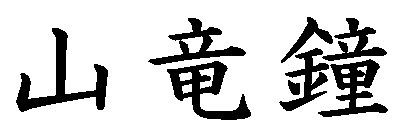
\includegraphics[width=2.75in]{./fig/yama-ryuu-kane.eps}
		\caption{Sample characters. The kanji ``yama'' (mountain), ``ry\=u'' (dragon), and ``kane'' (bell), written with 3, 10, and 20 strokes, respectively.}
		\label{fig_kanji_sample}
	\end{figure}

	\vfill


	\section{Problem description}
	\label{sec:problem_description}

	Any form of digital handwriting recognition is a complex undertaking,
	where the performance of the system is impacted by a multitude of factors -- spanning
	everything from the quality and quantity of training data, to resilience toward input
	translation, rotation, and noise. As the number of candidate categories increase
	the size of the search space, however, the task quickly grows monumental.

	The Japanese writing system consists of the two \emph{kana} syllabaries \emph{hiragana} and \emph{katakana},
	as well as the sinographs commonly known as \emph{kanji} -- literally ``Han characters'' -- that stem from China.
	The Japanese Ministry of Education's official ``regular use'' (j\=oy\=o) kanji list defines a set of 2,136
	baseline characters taught in elementary-- and secondary--school education. \cite{hadamitzky2012japanese}
	This set is far from exhaustive, though: the Japanese Industrial Standard X 0208 encoding, for instance, contains 6,355 different kanji.

	Although the characters are vast in number and differ significantly from one another in terms of complexity (see figures \ref{fig_kanji_sample}
	and \ref{fig_kanji_stroke_hist}), the writing system itself is not arbitrary. Any kanji may be broken down into smaller units, known as graphemes, 
	and they are commonly ``classified'' by basic, frequently--ocurring components referred to as radicals.
	Furthermore, stroke order is dictated by a set of rules. In essence, kanji are written from top to bottom and left to right within imagined squares. \cite{foerster1994kanji}

	These properties are often leveraged in kanji recognition systems, but not without penalty: relying on the correct stroke order during online
	recognition, for instance, severely impacts recognition rates when a user provides ``erroneous'' input -- even though it might still be \emph{visually} correct. \cite{shin2002optimal}

	While certain aspects such as noise reduction and normalization remain similar across systems, the characteristics mentioned above result in
	recognition systems designed for western input not performing satisfactorily when applied to asian script \cite{jager2003state, tappert1990state, liu2004online}
	-- unless the solution relies on complex techniques such as  ``deep'' neural networks. \cite{ciresan2012multi}


	%Given that the category search space for Japanese characters is an order of magnitude larger and contains a vastly differing set of
	%characteristics than its western counterparts, the same designs that yield highly accurate results on 
	%western handwriting recognition tasks do not perform satisfactorily when applied to asian script \cite{jager2003state, tappert1990state, liu2004online}
	%-- unless the solution relies on complex and computationally expensive techniques, such as  ``deep'' neural networks. \cite{ciresan2012multi}


	\begin{figure}
		\centering
		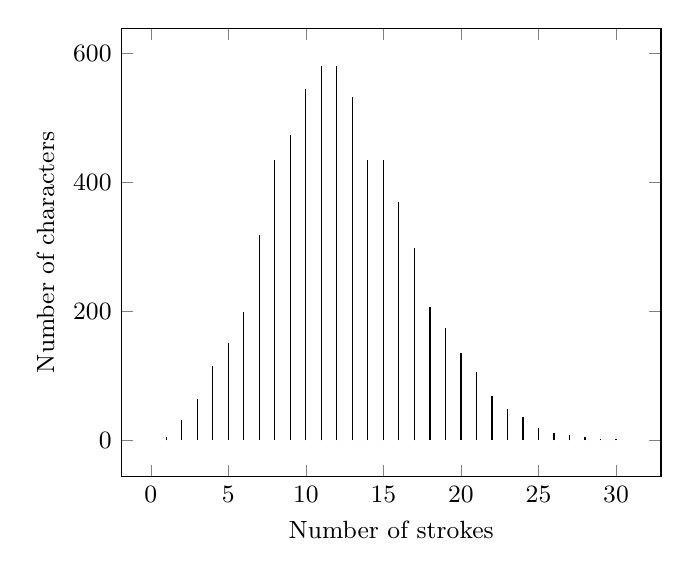
\begin{tikzpicture}[font=\small]
			\begin{axis}[
				ycomb,
				xlabel={Number of strokes},
				ylabel={Number of characters},
			]
				%\addplot[fill=white] coordinates {
				\addplot [] coordinates {
					(1, 6)
					(2, 32)
					(3, 64)
					(4, 115)
					(5, 151)
					(6, 199)
					(7, 318)
					(8, 434)
					(9, 473)
					(10, 544)
					(11, 581)
					(12, 581)
					(13, 532)
					(14, 435)
					(15, 434)
					(16, 369)
					(17, 299)
					(18, 207)
					(19, 175)
					(20, 135)
					(21, 106)
					(22, 69)
					(23, 49)
					(24, 37)
					(25, 20)
					(26, 12)
					(27, 8)
					(28, 6)
					(29, 3)
					(30, 2)
				};
			\end{axis}
		\end{tikzpicture}
		\caption{Distribution of 6,400 kanji by stroke count. Min = 2, Max = 581. \emph{Data source: KanjiVG.} \cite{kanjivg}}
		\label{fig_kanji_stroke_hist}
	\end{figure}



	\section{Previous work}
	\label{sec:previous_work}

	A vast body of work has been amassed on the topic of Japanese handwriting recognition.
	Here we summarize some notable publications that influenced our adopted approach.


	In \cite{joe1989large}, Mori and Joe present ``selective'' and ``integrative'' neural networks that 
	segment categories into small groups, thereby improving the recognition rate of each network.

	
	After structuring the search space by clustering, Yang et. al. perform two--stepped offline recognition by first
	comparing the input character to the centroids of each cluster, and then distinguishing between the members of the cluster
	whose centroid most closely matched the input. \cite{yang2003accelerating}


	In \emph{Hybrid Pen--Input Character Recognition System Based on Integration of Online--Offline Recognition},
	the authors present a system that leverages the advantages provided by each type of recognition.
	In addition to a discussion of various integration techniques, two feature extraction methods are described in detail: 
	a gradient--based technique for offline input, and a recursive substroke extractor for online input.


	% Got A-H classification from here
	In \cite{nakai2001substroke}, the authors adapt a continuous speech recognition algorithm utilizing
	hidden Markov models for the purpose of online kanji recognition. Captured strokes are segmented into
	substrokes and classified based on directionality (see figure \ref{fig_stroke_categories});
	the result is thereafter employed as dictionary search keys.


	\emph{Online Handwritten Kanji Recognition Based on Inter--Stroke Grammar} explains the hierarchical structure of kanji,
	and explores how to leverage this information using stochastic context--free grammars. \cite{ota2007online}

	Finally, albeit not directly applied to Japanese handwriting recognition, \emph{Best Practices for Convolutional Neural Networks
	Applied to Visual Document Analysis} by Simard, et. al. underlines the potential of convolutional neural networks 
	and provides a variety of techniques and guidelines directly applicable to the development of a fine--grain classifier. \cite{simard2003best}


	\begin{figure}
		\centering
		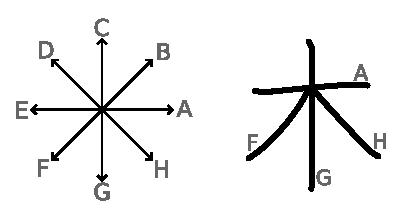
\includegraphics[width=1.75in]{./fig/stroke-categories.eps}
		\caption{A stroke may be classified according to its directionality.
			Further classes may be used to differentiate between long and short strokes,
		or to accomodate for ``pen--up'' motions. Here, the strokes of the kanji ``ki'' (tree) are identified as A-G-F-H.}
		\label{fig_stroke_categories}
	\end{figure}



	\section{Proposed solution}
	\label{sec:proposed_solution}

	Taking into consideration the issues presented in section \ref{sec:problem_description}
	%the problem posed by the large number of candidates, the characteristics of the kanji writing system,
	and the many influential works reviewed in section \ref{sec:previous_work}, we attempt to define a general description of a flexble, modular 
	design scheme that splits the identification task into coarse and fine phases -- thereby reducing the complexity of each undertaking -- and 
	additionally permits replacing the normalization, segmentation, and classification strategies.%, and facilitates the parallelization of fine classification.
	The design is applicable to online as well as offline recognition tasks.

	\begin{figure}[b]
		\centering
		
\includegraphics[width=2.75in]{./fig/model-overview.eps}
		\caption{The model consists of five components: input normalization methods, a feature extractor,
			a clustering strategy, a router (coarse classifier), and a fine--grained classifier.}
		\label{fig_model_overview}
	\end{figure}


	
	\subsection{Input normalization}

	Improving the input data, especially by making it more uniform with respect to available training data, has the potential
	to greatly increase recognition rates. In the case of offline input, techniques include noise--reduction,
	cropping, and scaling; for online input, strokes could be analyzed and altered on--the--fly to increase consistency.
	Other possibilities include blurring or otherwise distorting input data in order to generalize it. \cite{razzak2009combining}



	\subsection{Feature extraction}

	The feature extraction algoritm should take either online, offline, or combined input and rapidly generate
	an n--dimensional vector representation of the provided data. The output should be sufficient for the
	routing component to reliably distinguish within which candidate subset the fine classifier should search.

	Generally speaking, a higher feature vector dimensionality would allow for the construction of more finely--tuned clusters,
	but this might well increase the likelihood of misrouting.%, resulting in a failed classification.
	% Actually, if a character is not found within the specified CANN, it could be passed to a neighboring cluster of similar composition

	Examples of feature extractors include recursive substroke segmentation and image gradation, both outlined in \cite{tanaka1999hybrid}.



	\subsection{Category clustering}

	By structuring the search space into mutually exclusive clusters of similar categories,
	we are able to construct a corresponding number of fine classifiers that need only distinguish
	between the categories within its own cluster. The smaller search space directly translates into a
	significant reduction of model complexity, which in turn implies both a decrease in training time
	and the possibility of higher accuracy rates. Furthermore, given that no category overlap exists
	between the clusters, each fine classifier may be trained in parallel, and each model may be gradually
	improved as new training data is made available.



	As is proven in \cite{drineas2004clustering}, this is an NP-hard problem even in the case of $k = 2$. 

	Centroid-based clustering
	"Seeks to minimize the average squared distance between points in the same cluster"
	goal is to choose k centers so as to minimize $\varphi$, the total squared distance between each point and its closest center.

	\subsection{Feedforward routing network}


	\subsection{Convolutional character classification network}


	\section{Experiments}
	\label{sec:experiments}

	This will be a short section\ldots
	Describe the simple online feature extractor and following clustering scheme.

	\begin{figure}
		\centering
		
\includegraphics[width=2.75in]{./fig/experimental-implementation.eps}
		\caption{Experimental implementation. The input is first analyzed by the coarse classifier, resulting in the G-H-A\ldots feature representation.
		Thereafter, the routing network selects which cluster to search in, and the image data is passed to the corresponding CANN for fine--grain classification.}
		\label{fig_experimental_implementation}
	\end{figure}



	\subsection{Data sources}

	KanjiVG \ldots


	\subsection{Feature extraction}

	Figure of A-H compass. Explanation.

	\begin{table}
		\renewcommand{\arraystretch}{1.3}
		\caption{Stroke type frequency distribution overview }
		\label{tbl_stroke_analysis}
		\centering
		\begin{tabular}{ c | c c c c c l }
			\hline
			  & \bfseries \% & \small $\sum$ & $\mu$ & $\sigma$ & Highest count \\ 
			\hline
			\hline
			\bfseries A & $33.20\%$ & $26,160$ & $4.09$ & $2.33$ & $15$ & \\%(蠶) \\
			\bfseries B & $1.47\%$  & $1,159$  & $0.18$ & $0.40$ & $2$  & \\%(摑) \\
			\bfseries C & $0.00\%$  & $0$      & --     & --     & --   & \\%     \\
			\bfseries D & $0.00\%$  & $0$      & --     & --     & --   & \\%     \\
			\bfseries E & $0.31\%$  & $245$    & $0.04$ & $0.19$ & $2$  & \\%(霪) \\
			\bfseries F & $12.72\%$ & $10,018$ & $1.57$ & $1.36$ & $10$ & \\%(鏐) \\
			\bfseries G & $29.98\%$ & $23,616$ & $3.69$ & $1.96$ & $13$ & \\%(鱸) \\
			\bfseries H & $22.32\%$ & $17,587$ & $2.75$ & $1.61$ & $11$ & \\%(靆) \\
			\hline
			            & $100.00\%$   & $78,785$ &        &        &      & \\
			\hline
		\end{tabular}
	\end{table}



	\subsection{Clustering}

	Whereas in \cite{nakai2001substroke} strokes were segmented into substrokes and classified in
	25 dimensions, our initial feature extraction strategy provides a coarse full--stroke classification
	in 8 dimensions. By discarding ``pen--up motions,'' we render the system more resilient to erroneous
	stroke order, at the cost of increasing variability within each cluster.


	\ldots decided to consider the value given by the ``rule of thumb'' $k \approx \sqrt{n / 2}$ proposed in \cite{mardia2005multivariate}
	as an upper limit to the number of clusters.

	$$ k_{max} = \sqrt{6,396 / 2} \approx 57 $$

	The clusters were generated using the k--means++ algorithm,
	a variation of Lloyd's algorithm that seeks to improve the selection of the initial centroids. \cite{arthur2007k}

	Based on the information summarized in table \ref{tbl_stroke_analysis}, \ldots

	\begin{table}
		\renewcommand{\arraystretch}{1.3}
		\caption{Some form of cluster sample}
		\label{tbl_sample_clusters}
		\centering
		\begin{tabular}{c}
			We could list centroid info and some sample kanji. \\
			But not \emph{all} the clusters, right? Too many\ldots \\
		\end{tabular}
	\end{table}



	%\begin{tikzpicture}[font=\small]
	%	\begin{axis}[
	%		ybar,
	%		bar width=20pt,
	%		xlabel={Stroke feature classification},
	%		ylabel={Frequency (\%)},
	%		ymin=0,
	%		ymax=40,
	%		%ytick=\empty,
	%		xtick=data,
	%		axis x line=bottom,
	%		axis y line=left,
	%		enlarge x limits=0.2,
	%		symbolic x coords={A, B, C, D, E, F, G, H},
	%		xticklabel style={anchor=base, yshift=-\baselineskip},
	%		nodes near coords={\pgfmathprintnumber\pgfplotspointmeta}
	%	]
	%		\addplot[fill=white] coordinates {
	%			(A, 33.2)
	%			(B, 1.5)
	%			(C, 0)
	%			(D, 0)
	%			(E, 0.3)
	%			(F, 12.7)
	%			(G, 30.0)
	%			(H, 22.3)
	%		};
	%	\end{axis}
	%\end{tikzpicture}

	\section{Preliminary results}
	\label{sec:experiment_results}

	Not done yet, but here we go.


	\section{Conclusions}
	\label{sec:conclusions}

	This work is cool, now give complimentary M.Sc. plx?
	They did it for Donald Knuth\ldots :(


	\section{Future work}
	\label{sec:future_work}

	The experimental results documented in this paper are an initial attempt at applying the proposed methodology;
	numerous variations remain to be explored. With regard to online recognition, the explored feature extraction
	strategy could be enhanced to break strokes into substrokes, diffentiate between long and short strokes, and take
	pen--up movements into account. This alteration would in turn allow clustering on up to 25 dimensions, rather than the current 8.

	By substituting the current coarse classifier with an offline feature extraction strategy, the entire system could
	be evaluated on offline handwriting recognition datasets, such as\ldots. 

	Clustering\ldots

	Finally, at the cluster--specific CANN--level, there is ample opportunity to tweak the network topology as well as
	to apply a variety of best practices \cite{simard2003best} in order to enhance the final, fine--grain recognition results.



	% References
	\bibliography{./references}

\end{document}
